\chapter{Tanulásmenedzsment rendszerek IT infrastruktúrája}
\section{A három rétegű architektúra}
A webes LSM-ek általában a három rétegű architektúrát követik. Ez a három réteg a webkiszolgáló, az adatbázis és az alkalmazás réteg. A réteges szerkezetnek köszönhetően ezek a rendszerek jól skálázhatóak, hiszen az egyes rétegekben megtalálható szolgáltatásokat gyakran ilyen funkciókkal alakítják ki.
A rétegeknek nem szükséges fizikailag is külön hardverre kerülni (sőt az alkalmazás- és webkiszolgáló-réteg esetében ez  nem is mindig lehetséges), így a legegyszerűbb kialakítás akár egy számítógépet is igénybe vehet. Ez a megoldás egy viszonylag erős konfiguráció és alacsony felhasználószám esetén működhet.
\subsection{A webkiszolgáló-réteg}
\todo{Webszerver}
\subsection{Az alkalmazásréteg}
\todo{Alkalmazás szerver}
\subsection{Az adatbázisréteg}
\todo{DB}

És itt elő is kerül az elterjedtebb LMS-ek előnye: a könnyű telepítés, beüzemelés. Vegyük például

\section{Egy példa}
\subsection{A Moodle rendszer}
Az e-learning rendszerek közül a legelterjedtebb a Moodle (Modular Object-Oriented Dynamic Learning Environment) (\href{http://moodle.org}{http://moodle.org}) nevű tanulásmenedzsment rendszer. Önálló laboratóriumi munkám során ennek a rendszernek a részletesebb megismerése volt az egyik cél.

A Moodle  egy ingyenes és nyílt forrású LMS vagy VLE (Virtual Learning Environment, Virtuális oktató környezet). 2010 októberében 49952 regisztrált Moodle oldal létezett, amelyek összesen mintegy 37 millió felhasználót szolgáltak ki. A legnagyobb rendszertelepítések közé tartozik a tajvani Ming Chuan Egyetem több, mint 63.000 regisztrált, maximálisan 33.000 bejelentkezett felhasználóval naponta.

\todo{Forrás http://docs.moodle.org/20/en/Installations\_30000\_plus}

Maga a rendszer tervezéséből és implementálásából eredően portábilis, hála a PHP nyelvnek. Módosítás nélkül telepíthető Unix, Linux variánsokra, FreeBSD-re, Windows-ra, Mac OS X-re, NetWare-re és egyéb rendszerekre, amelyek támogatják a PHP-t és az ismertebb adatbázis-kezelő rendszereket.

A Moodle architektúrájában elválik a natív adatbázis-kezelő a felsőbb rétegektől. Közöttük egy ADOdb adatbázis absztrakciós réteg található. Az ADOdb egy különálló projekt (\href{http://adodb.sourceforge.net/}{http://adodb.sourceforge.net/}), amely a legelterjedtebb adatbázis-kezelőket támogatja. \Aref{fig:moodlearch}.~ábrán egy korábbi verzió architektúrája látható.

\begin{figure}[h!]
\centering
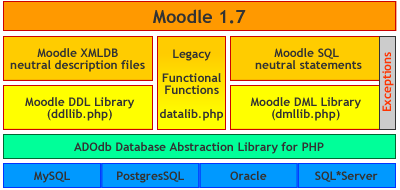
\includegraphics[width=0.8\textwidth]{figures/moodlearch.png}
\caption{A Moodle architektúrája \label{fig:moodlearch}}
\end{figure}

Az architekturális felépítésből látható, hogy a Moodle az ADOdb által nyújtott rétegen keresztül egységesen éri el az eltérő adatbázis megvalósításokat anélkül, hogy foglalkoznia kellene az ezekből eredő problémákkal.  

Az interoperabilitás több Moodle képességben megjelenik, ilyenek például:
\begin{itemize}
\item autentikáció LDAP-on, Shibboleth-en keresztül
\item kérdések/kérdéssorok importálása/exportálása több formátumban (pl. XML, XHTML stb.)
\item erőforrások kezelése (SCORM, AICC)
\item integráció más tartalom kezelő rendszerekkel (Drupal, Postnuke).
\end{itemize}

A Moodle fontos tulajdonsága a modularitás, vagyis a rendszer funkcionalitásának könnyű bővíthetőségek. Ezeket plug-inokkal valósítják meg, amelyek fejlesztését különböző API segítik. Ilyen plug-inok pl. a különböző jelentések (reportok), blokkok, portfóliók, tárolók (repository-k), kereső modulok. Ezek közül nagyon sok megtalálható az alap Moodle telepítésben is, de saját magunk is írhatunk hasonló kiegészítőket.

\subsection{A Moodle egy lehetséges infrastruktúra kialakítása}
